% ----------研究三
\chapter{研究三:基于文本特征与用户偏好的个性化广告效果模型构建}

相关研究表明,人格特质与语言表达模式之间存在密切关系,但这些研究成果主要来源于社交媒体等用户生成内容 (User-Generated Content, UGC) 领域 \citep{azucar2018predicting}。例如,有研究发现,高外向性个体在社交媒体中的语言风格通常更为积极且富有互动性,而高开放性个体则偏好多样、富有创造性的语言表达。此外,通过分析用户在社交媒体中的点赞、评论和转发行为,研究者能够有效预测用户的大五人格特质。这些研究不仅证实了人格特质与语言特征之间的紧密联系,也展示了语言风格在反映个体心理特质中的重要作用。然而,这种“人格-语言”关联是否同样体现在基于人格定制生成的广告文案中,仍然缺乏系统性验证。与社交媒体中的自然语言表达不同,广告文本具有传播目的明确、语言风格结构化等特点,其语言特征是否能够如社交媒体内容般准确反映目标人格特质,尚不明确。造成这一研究空白的重要原因在于传统实验中的广告样本数量有限,难以支撑大规模、多维度的人格-语言特征系统分析。以往研究往往依赖人类专家创作广告文本,样本规模小且创作风格易受主观偏好影响,难以全面揭示不同人格设定下广告语言特征的差异性。然而,随着生成式人工智能 (Generative AI, 如 GPT) 技术的快速发展,研究者得以突破这一限制。AI能够批量生成符合不同人格设定的大规模广告文本样本,并在生成过程中严格控制语言风格以匹配预设的人格特质。这不仅有效解决了传统研究中样本不足的问题,还为深入系统性分析广告文案中的人格语言特征提供了技术基础。

因此,为填补这一研究空白,本研究在前述实验探究的基础上,进一步从文本分析的角度对个性化广告的语言特征及其匹配效果进行深入探讨。借助前续实验中 AI 生成的大规模广告数据,研究三将系统分析不同人格特质广告文案的语言风格,并探讨其如何通过语言结构、情感表达和认知内容来实现个性化匹配。研究三包含两个子研究。子研究一利用 LIWC(Linguistic Inquiry and Word Count)等文本分析工具,对个性化广告进行语言特征分析,探讨不同人格特质广告文案在语言风格上的异同。子研究二则进一步结合这些语言特征数据和个性化广告的参与者评分,构建预测模型,以快速识别文本的个性化说服效果,并探索不同语言特征在个性化广告中的作用。这一研究不仅能够揭示个性化广告文本的语言模式,还能为AI生成广告的优化提供理论依据和实证支持,为未来广告设计和投放策略提供数据驱动的决策依据。

\section{子研究一:各人格特质的广告文案特征分析} 
\label{study3-substudy1}

\subsection{方法}
\label{LIWC}

\textbf{(1)实验材料}

在本研究的研究一与研究二中,共收集了145条基于大五人格模型(外倾性、开放性、尽责性、宜人性、神经质)定制生成的广告文案,覆盖了高水平与低水平人格特质的广告版本。然而,统计结果显示,145条广告中仅有8条为针对低水平特质设计的广告,样本量严重不足,难以对低水平特质的广告特征进行系统性分析。因此,为确保分析结果的科学性与代表性,当前聚焦于137条针对高水平人格特质(即高外倾、高开放、高尽责、高宜人和高神经质)设计的广告文案,通过定量文本分析深入探索不同人格特质广告文案的语言特征及其潜在模式。

\textbf{(2)分析方法}

本研究采用语言分析与词汇计算软件(Linguistic Inquiry and Word Count, LIWC)对137条广告文案进行文本特征分析。LIWC 是一款广泛应用于语言心理学、社会科学和计算传播学等领域的文本分析工具,由 Pennebaker 等人开发 \citep{pennebaker2007linguistic}。该工具通过内置的词典库对文本进行分类和统计,能够揭示文本的心理、情感及语言特征,其核心优势在于对语言风格和心理状态的多维度解析。LIWC 词库结构丰富,包含多个心理、情感和语言类别,涵盖数千个词根和语言表述单元。其分析维度包括但不限于情感类别、认知过程、社会过程和驱动因素等。情感类别包括正面情感(positive emotion)和负面情感(negative emotion),用于衡量广告中情感诉求的特征;认知过程涵盖因果词(causation)、洞察词(insight)和不确定性词(tentative),反映广告内容是否引发消费者的思考与联想;社会过程涉及人称代词和社交行为词(social words),揭示广告是否具有社交导向或用户互动属性;驱动因素如成就词(achievement)、权力词(power)等,体现广告是否激发消费者的内在动机和购买意愿。

在分析过程中,本研究对每条广告文案进行了多维度文本特征提取,并对五种人格特质(外倾性、开放性、尽责性、宜人性、神经质)下的广告文案特征进行比较,重点关注各语言特征在五种人格维度上的差异。这一分析不仅有助于识别特定语言特征与某一人格特质水平之间的关联性,还为深入理解个性化广告中文案风格的特质匹配效应提供了定量依据。


\subsection{结果}

基于对137条针对高水平特质设计的广告文案的LIWC分析,从人格特质维度对各语言特征进行了统计分析。具体而言,我们计算了 LIWC 输出的 90 余个语言特征在五种人格(外倾性、开放性、尽责性、宜人性、神经质)之间的均值差异,并采用单因素方差分析 (One-way ANOVA) 检验这些语言特征在不同人格特质广告中的显著性差异,结果如图\ref{fig:Study3-LIWC}所示。

\begin{figure}[htbp]
    \centering
    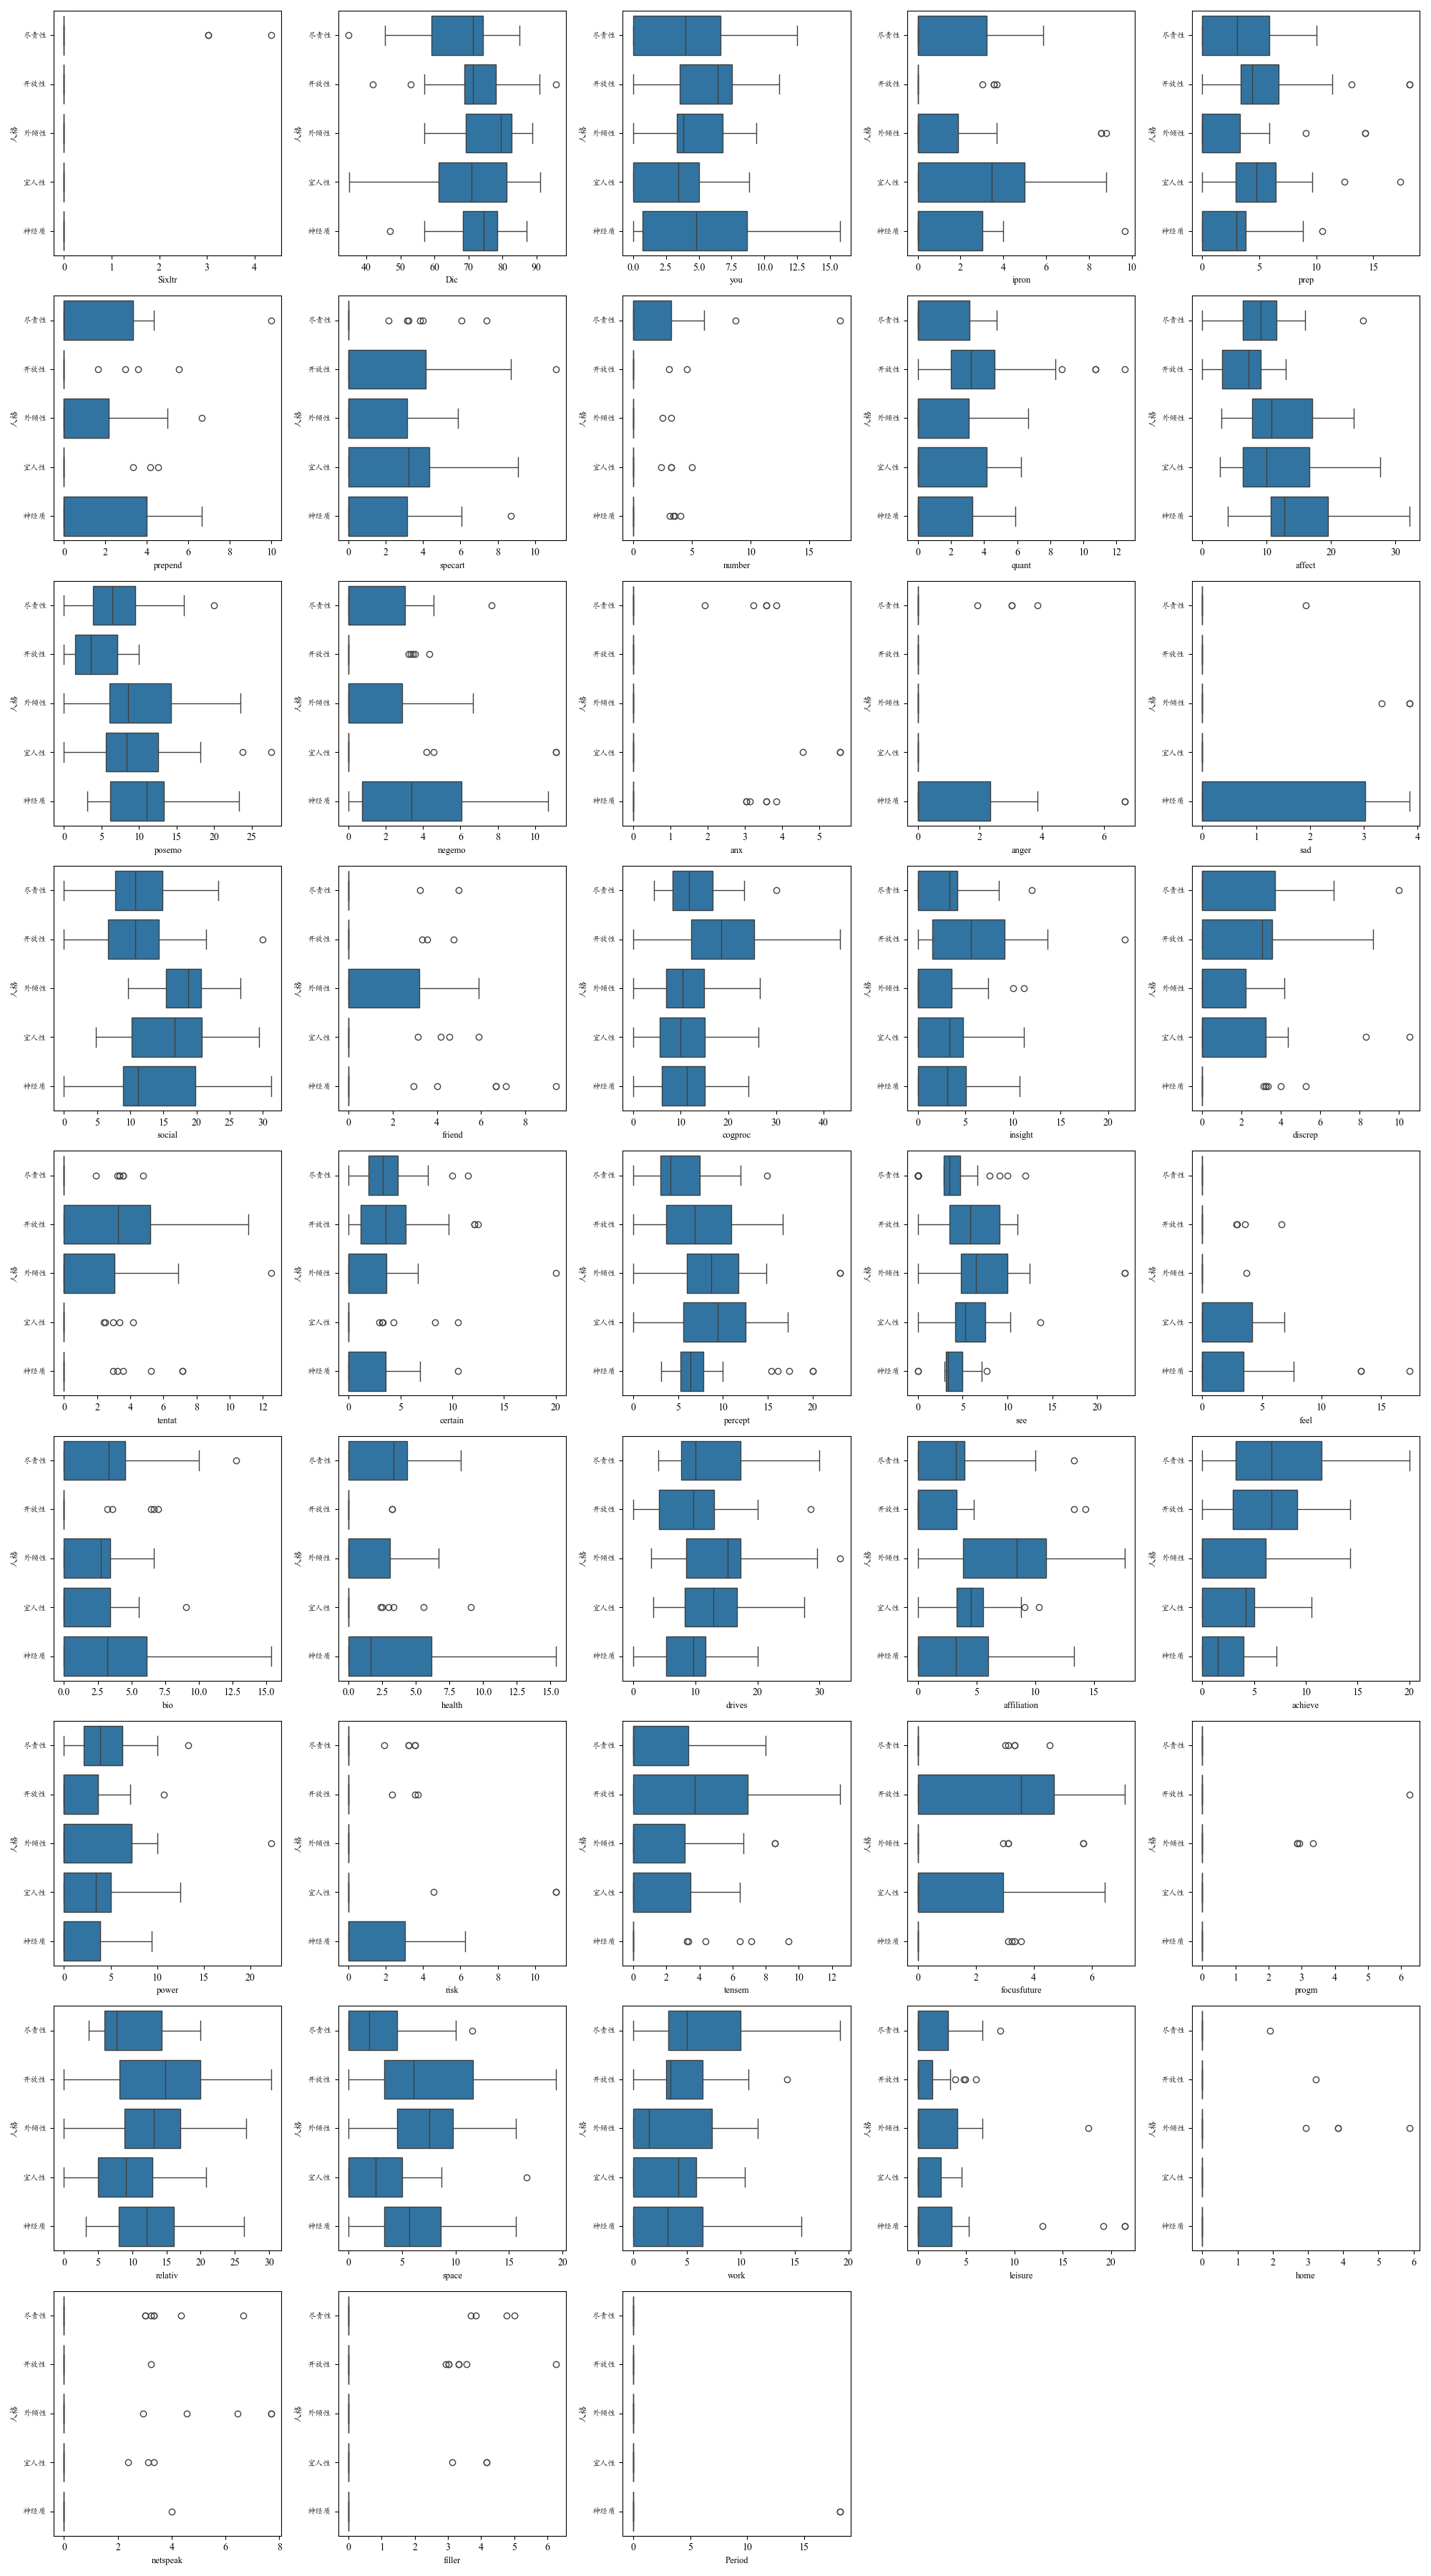
\includegraphics[width=0.8\linewidth]{Image/Study3-LIWC.png}
    \caption{\label{fig:Study3-LIWC}基于大五人格特质的个性化广告文本的语言特征分布}
\end{figure}

\textbf{外倾性}广告语言突出社交性与情感表达,符合外倾性人格的活跃与互动特质。外倾性广告中的社交相关词(social, \textit{F}(4,132) = 6.360, \textit{p} = 0.0001, 18.17\%)和归属动机词(affiliation, \textit{F}(4,132) = 9.840, \textit{p} < 0.001, 7.72\%)显著高于其他人格特质,体现出强烈的社交导向。此外,外倾性广告中的正面情感词(posemo, \textit{F}(4,132) = 7.181, \textit{p} < 0.001, 10.35\%)和感知词(percept, 9.32\%)的比例均为最高,进一步突出了积极、外向和注重体验的语言风格。

\textbf{宜人性}广告语言突出了情感温度和人际联结,体现了宜人性人格的共情与亲和特质。宜人性广告在正面情感词(posemo, 9.71\%)、社交相关词(social, 15.58\%)和归属动机词(affiliation, 4.75\%)方面均有较高占比,显示出广告内容偏向温暖、友好和关怀。此外,宜人性广告的语言风格也较为柔和,使用更多的情感相关词(affect, \textit{F}(4,132) = 8.942, \textit{p} < 0.001, 11.37\%)来增强情感连接。

\textbf{尽责性}广告语言风格注重目标导向和逻辑性,凸显了尽责性人格的计划性与成就驱动力。高尽责性广告中成就动机词(achieve, \textit{F}(4,132) = 6.710, \textit{p} = 0.0001, 7.32\%)使用最多,符合尽责性人格对成功和结果导向的关注。此外,尽责性广告在长词使用率(Sixltr, \textit{F}(4,132) = 2.898, \textit{p} = 0.0245)和数量词使用率(quant, \textit{F}(4,132) = 6.061, \textit{p} = 0.0002)上也显著高于其他特质,表现出语言上的正式性和条理性。

\textbf{开放性}广告文案呈现出鲜明的探索性与认知导向特征。高开放性广告在认知加工词(cogproc, \textit{F}(4,132) = 7.442, \textit{p} < 0.001, 19.60\%)和洞察词(insight, \textit{F}(4,132) = 3.829, \textit{p} = 0.0056, 5.93\%)的使用比例显著高于其他人格特质,反映了开放性人格偏好深入思考与探索的特质。此外,开放性广告大量使用空间相关词(space, \textit{F}(4,132) = 6.550, \textit{p} = 0.0001, 7.19\%)与感知词(percept, \textit{F}(4,132) = 3.321, \textit{p} = 0.0125, 7.74\%),表现出强调体验、探索与审美感知的语言风格。

\textbf{神经质}广告语言表现出显著的情绪波动与情感敏感特征。神经质广告中负面情感词(negemo, \textit{F}(4,132) = 7.308, \textit{p} < 0.001, 3.84\%)、焦虑词(anx, \textit{F}(4,132) = 2.845, \textit{p} = 0.0266, 0.78\%)、愤怒词(anger, \textit{F}(4,132) = 6.394, \textit{p} = 0.0001, 1.19\%)和悲伤词(sad, \textit{F}(4,132) = 8.058, \textit{p} < 0.001, 1.15\%)的使用均显著高于其他人格特质。这种情绪化的表达不仅强化了情感连接,也反映了神经质个体对情绪体验的高度敏感性。


在 LIWC 分析基础上,我们进一步通过词云图(图 \ref{fig:Study3-wordCloud})展示了五种人格特质广告的高频词。在制作词云图时,为突出各人格特质广告在语言风格上的差异,我们首先对五种人格个性化广告文本进行了预处理。具体而言,剔除了广告文本中未能体现人格特征且具有广泛通用性的高频词,例如“手机”“我们”“智能”等通用词汇。这些词语虽在广告中频繁出现,但主要源于广告语境和产品描述,与人格特质无直接关联,保留反而会掩盖不同人格特质在语言特征上的差异性。词云图中词语的大小代表其在对应人格广告中的出现频率,直观反映了各人格特质广告在语言风格上的差异。针对\textbf{外倾性}的广告,突出社交体验与分享感,词云中高频词如\textbf{“世界”“朋友”“分享”}与LIWC 中社交词(social)类别的高频结果一致,充分体现了外倾性个体偏好社交和互动的特质。\textbf{宜人性}广告强调情感共鸣与温暖体验,\textbf{如“美好”“温暖”“陪伴”}与 LIWC 中积极情感词(posemo)类别的高频结果相符,符合宜人性人格重视人际和情感连接的特点。\textbf{尽责性}广告则突出了功能性和可靠性,词云中的\textbf{“精准”“高效”“细节”}与 LIWC 中成就动机词(achieve)和认知加工词(cogproc)类别一致,契合尽责性人格偏好条理性和目标导向的特征。\textbf{开放性}广告则体现了探索与创造性的主题,高频词如\textbf{“创意”“探索”“无限”}与 LIWC 中感知类(percept)和洞察类词(insight)的高频结果相符,反映了开放性人格追求新体验和创造力的偏好。\textbf{神经质}广告则着重于情感安抚与安全感,\textbf{“陪伴”“温暖”“放松”}如,与 LIWC 中负面情感词(negemo)、焦虑词(anx)及亲和性词(affiliation)的显著性结果一致,突出了神经质人格在情绪波动中对安全感和情感支持的需求。

综合 LIWC 分析与词云可视化结果,本研究揭示了不同人格特质广告在语言特征上的显著差异,充分展现了基于大五人格模型的个性化广告语言模式。这一结果不仅丰富了对个性化广告语言特征的理解,也进一步验证AI基于人格特征生成个性化广告文本的能力。

\begin{figure}[H]
    \centering
    % 第一行三张图
    \subfloat[外倾性]{
        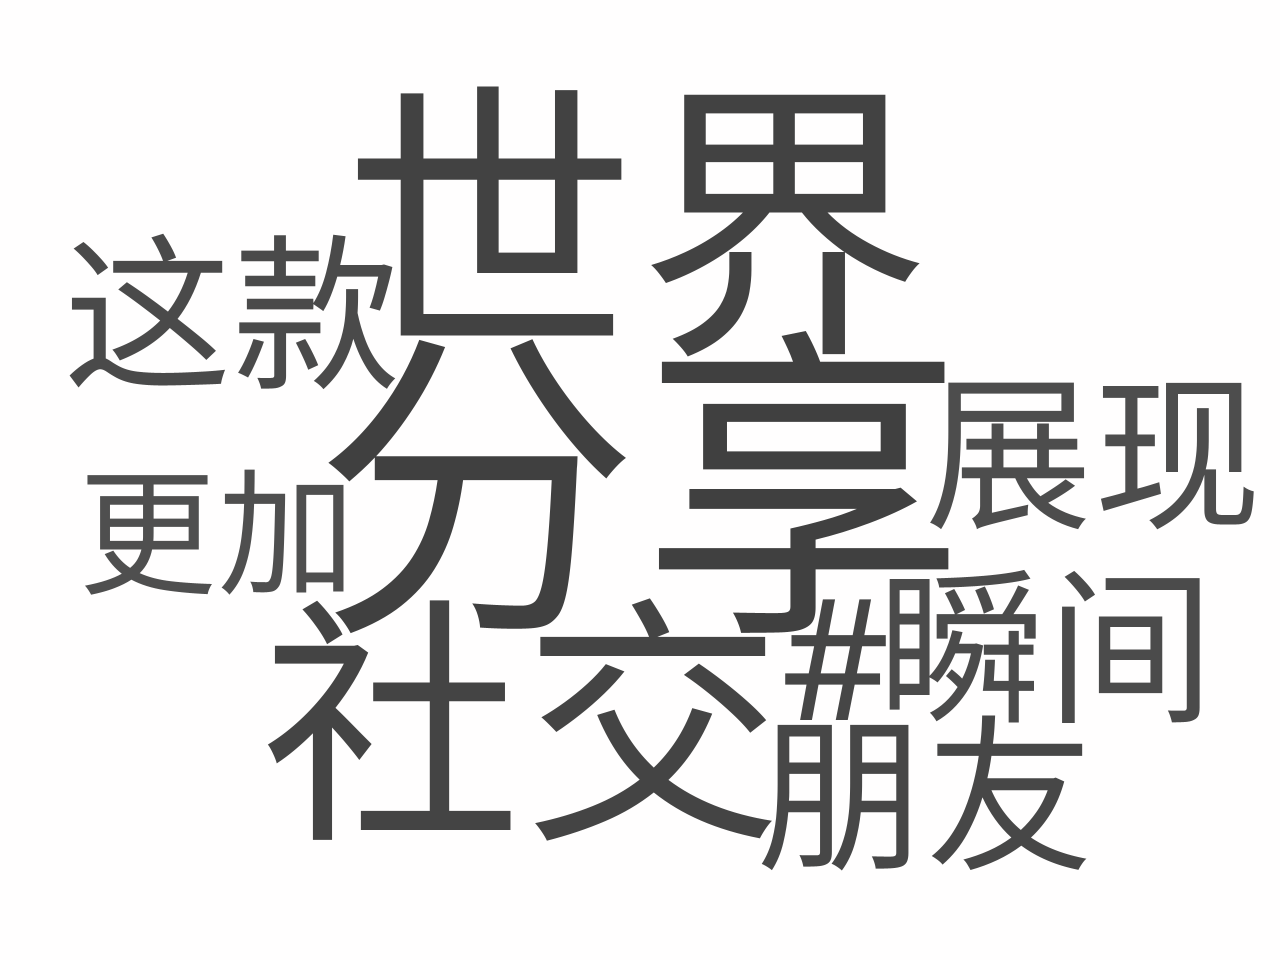
\includegraphics[width=0.2\linewidth]{Image/Study3-外倾性.png}
    }\hspace{1em}
    \subfloat[宜人性]{
        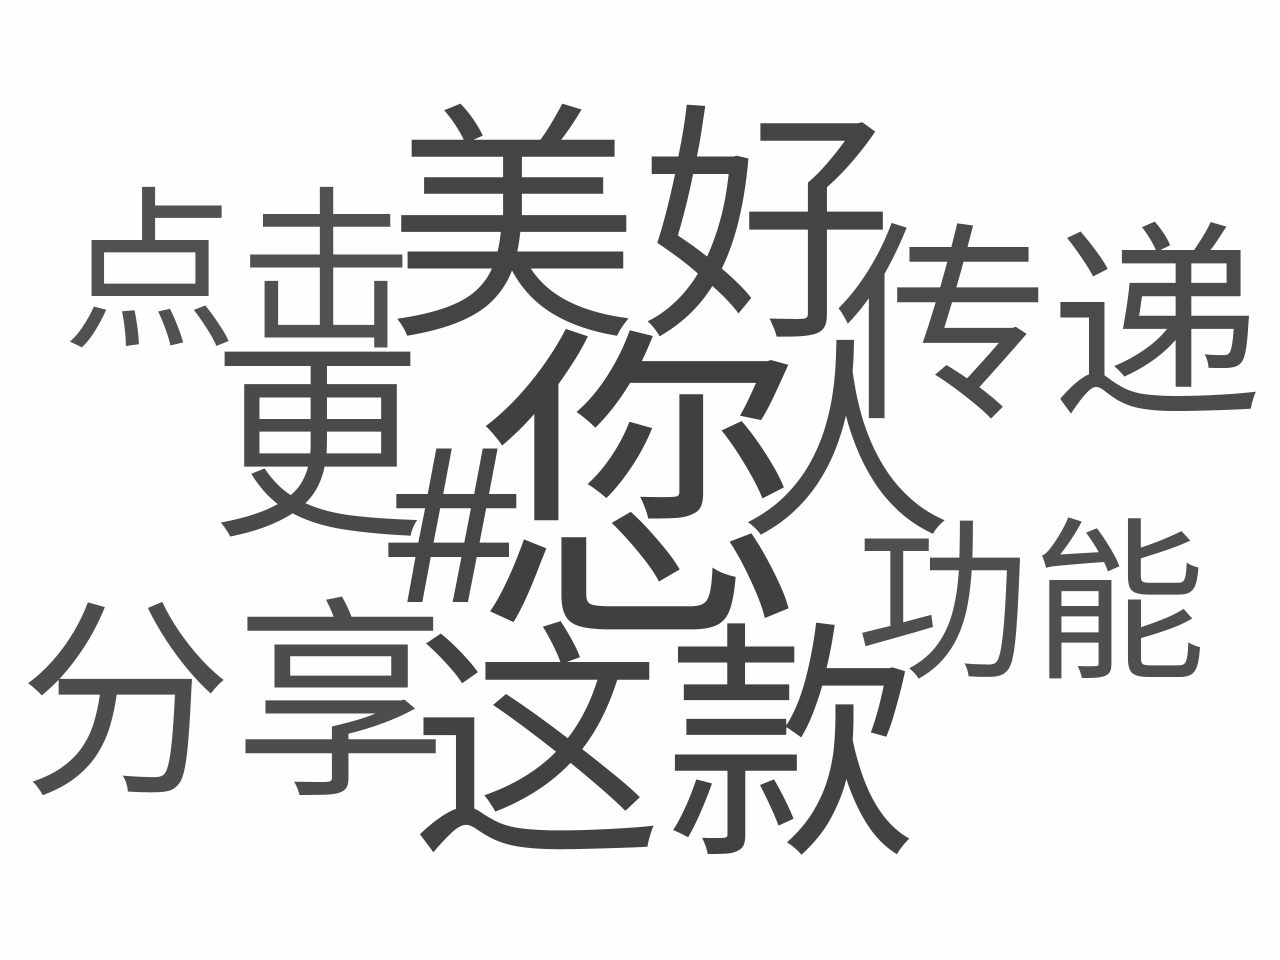
\includegraphics[width=0.2\linewidth]{Image/Study3-宜人性.png}
    }\hspace{1em}
    \subfloat[尽责性]{
        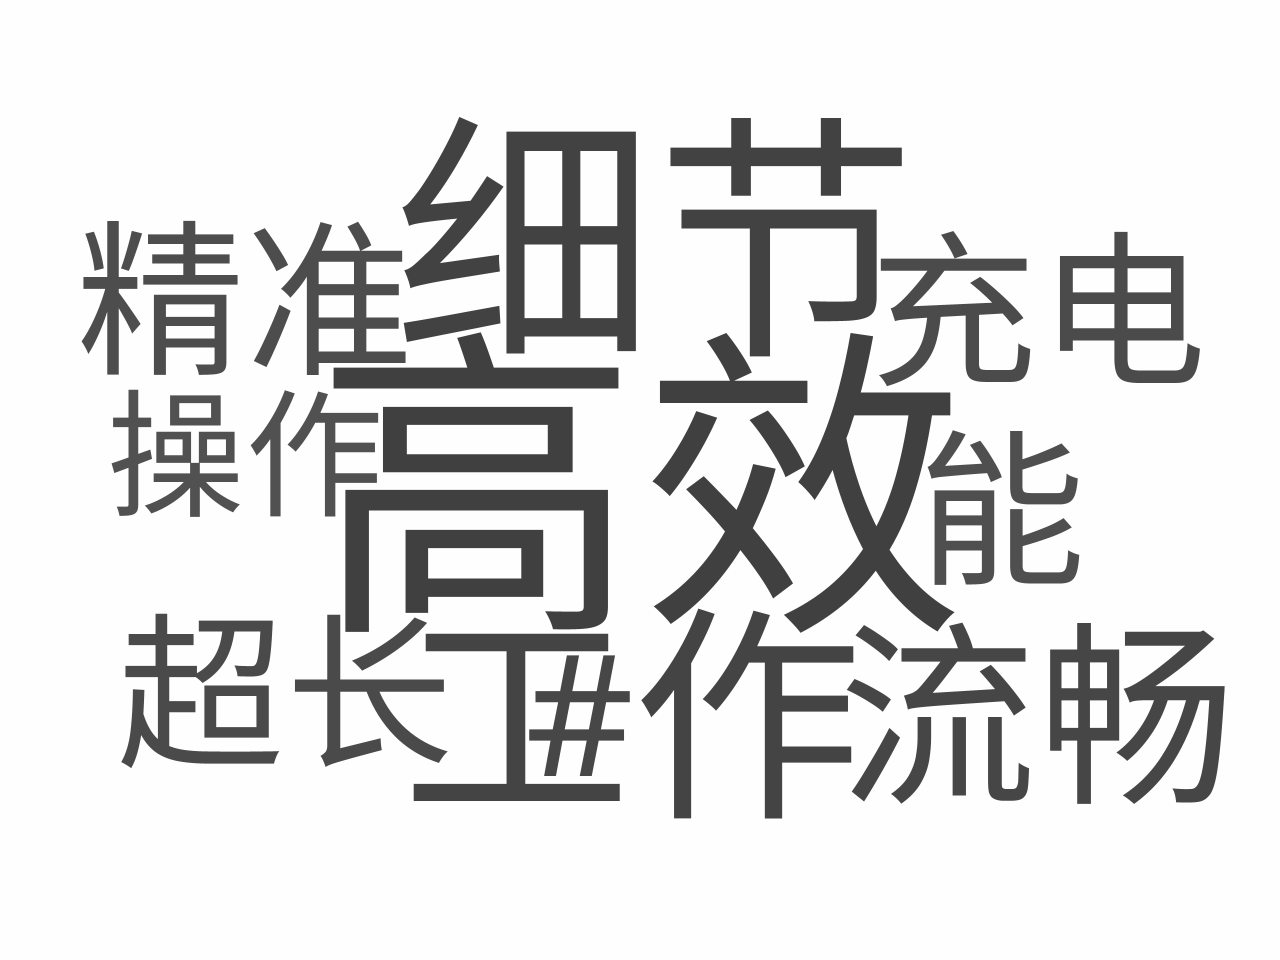
\includegraphics[width=0.2\linewidth]{Image/Study3-尽责性.png}
    }
    \\[1em] % 换行并增加垂直间距
    % 第二行两张图
    \subfloat[开放性]{
        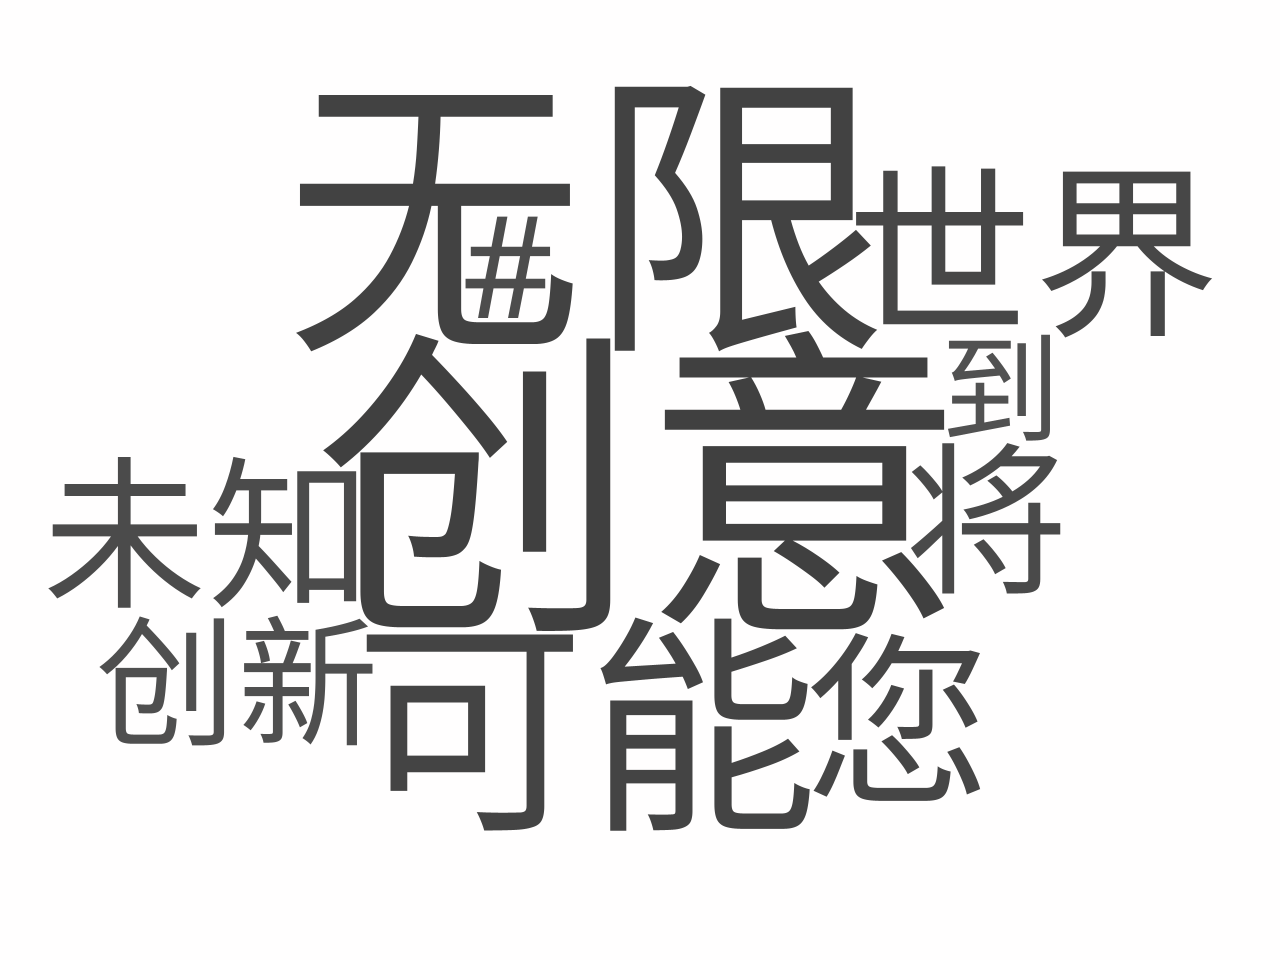
\includegraphics[width=0.2\linewidth]{Image/Study3-开放性.png}
    }\hspace{2em}
    \subfloat[神经质]{
        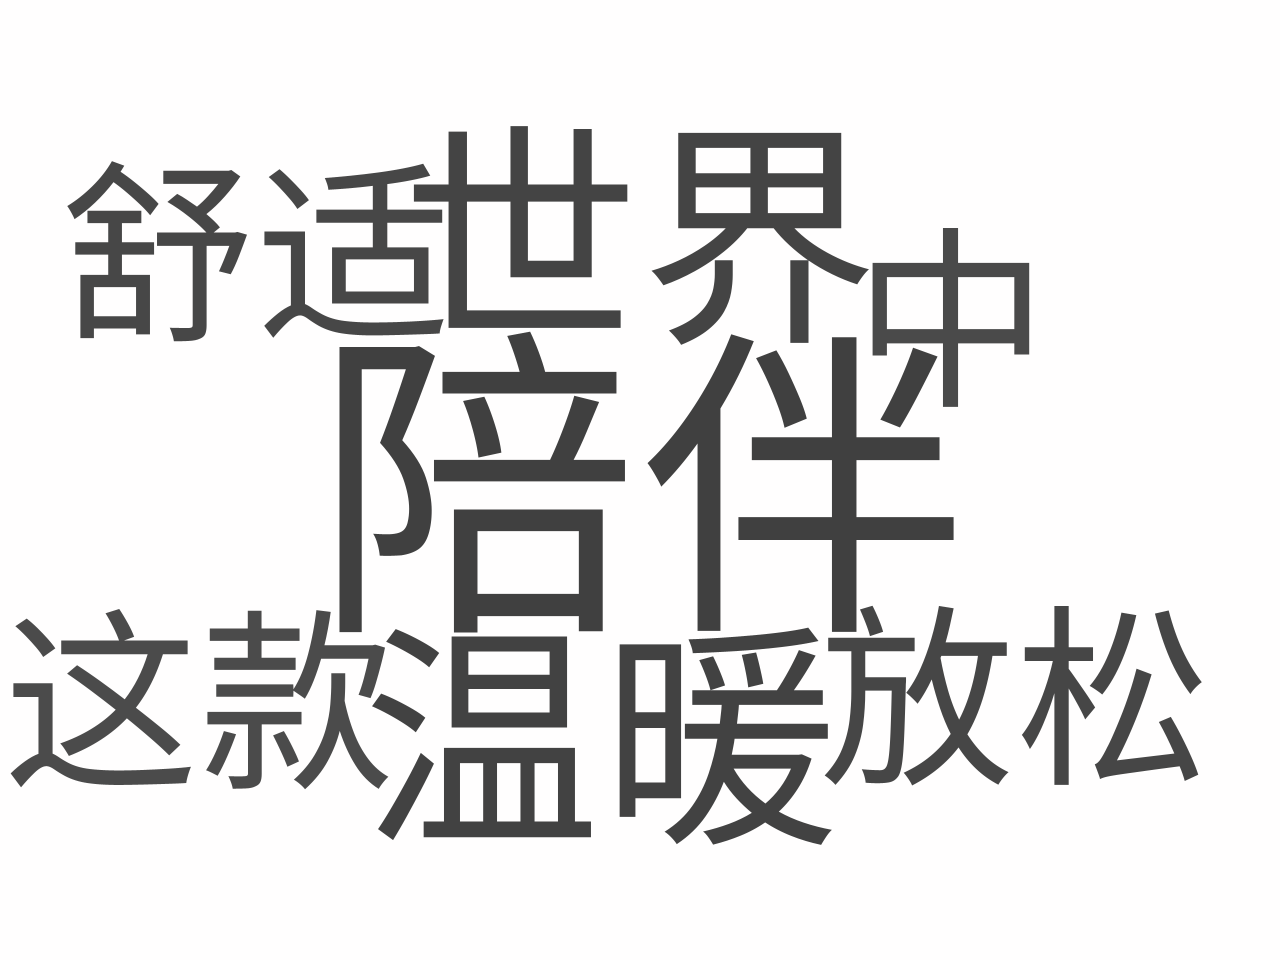
\includegraphics[width=0.2\linewidth]{Image/Study3-神经质.png}
    }
    \caption{\label{fig:Study3-wordCloud}基于大五人格特质的个性化广告文本词云图}
    \label{fig:personality_images}
\end{figure}


\section{子研究二:个性化广告效果模型构建} 
在研究一和研究二中,个性化广告的效果评估主要依赖实验数据。尽管 AI 生成技术显著降低了实验材料的制作成本,使大规模生成个性化广告成为可能,但广告效果的验证仍需大量被试,并要求他们填写人格问卷,以匹配个性化广告的目标群体。然而,这种基于实验的方法不仅在时间和资源上存在限制,难以实现快速评估,还需要依赖受试者的参与,因而在实际应用中具有一定局限性。因此,构建预测模型能够提供一种更高效的评估手段,使研究者或广告实践者在广告发布前预测其对不同人格特质群体的吸引力。这不仅有助于降低实验成本,还能在广告投放前优化个性化策略,从而提高广告匹配度和转化率。此外,在前述研究中,我们已收集了大量基于 AI 生成的广告文本,并获得了带有个性化特质信息的被试评分数据,使得构建个性化广告说服效果模型成为可能。尽管实验中的广告是围绕某一特定人格特质(如高外倾性、高开放性等)进行定制的,但广告文本可能包含多层次的语言元素,使其不仅对目标特质群体有效,也可能吸引其他人格特质的个体。例如,一个为高开放性个体设计的广告可能突出探索性与创造力,但其中的情感化或社交化表达同样可能对高宜人性或高外倾性的个体产生吸引力。因此,在模型构建过程中,我们不仅考察广告在目标特质群体中的说服效果,还计算该广告对其他人格特质个体的吸引程度。这一方法突破了传统个性化广告评估仅关注目标群体的局限,使得模型能够更全面地预测个性化广告在不同人格特质群体中的适用范围,为广告优化和投放策略提供更具适应性的参考。综上所述,子研究二基于前述实验的实验材料和数据,结合LIWC语言特征,构建个性化广告效果的预测模型。

\subsection{方法}

\subsubsection{建模数据}

\textbf{(1)数据来源}

本研究的模型构建基于研究一和研究二的实验数据,涵盖 AI 生成与人类专家创作的个性化广告文本及其参与者评分。所有实验均采用大五人格测量工具(BFI-10 或 BFI-44)评估参与者的人格特质,并要求他们对不同个性化广告文本进行评分。为确保模型能够准确评估广告对不同人格特质群体的吸引力,我们优先选取完成完整人格测量的实验数据,以提高个性化说服效果计算的精度。具体而言,模型训练数据整合了多个实验的数据集(详见表 \ref{tab:model_data}),每名参与者在实验中评价 5 条广告,而每条广告的最终评价人数因实验条件不同而有所变化。经过筛选,最终用于模型训练的广告样本共计112条。

\begin{table}[htbp]
    \centering
    \caption{\label{tab:model_data} 建模数据来源}
    {\tablesongti % 整个表格环境应用宋体六号字体
    \renewcommand{\arraystretch}{1.5} % 调整行距
    \begin{tabular}{p{2cm} p{2cm} c c c} % 控制列宽
        \toprule
        \textbf{实验} & \textbf{人格测量量表} & \textbf{参与者人数} & \textbf{每名受试者评价文本数} & \textbf{单条广告评价人数} \\
        \midrule
        研究一-实验1 & BFI-10 & 192 & 5 & 65 \\
        研究二-实验1 & BFI-10 & 322 & 5 & 32--59 \\ % 使用 -- 代替 –
        研究二-实验2 & BFI-44 & 368 & 5 & 13--68 \\ % 使用 -- 代替 –
        \bottomrule
    \end{tabular}
    }
\end{table}




\textbf{(2)计算方法}
\label{calculationMethods}

为构建模型,我们对个性化广告的说服效果进行了量化处理。计算过程分为\textbf{个体层面}和\textbf{广告层面}。

在\textbf{个体层面},我们首先对每名受试者在实验中的广告评分进行标准化,以消除个体评分偏差。随后,将个体的人格得分也进行标准化,并计算个体在所有广告上的评分与其在人格上的偏离程度,以衡量特定人格水平个体对广告的偏好倾向。具体计算如下,其中,\( S_{\text{ad},i} \) 代表个体 \( i \) 在某条广告上的评分,\( \mu_{S,i} \) 和 \( \sigma_{S,i} \) 分别为该个体在所有广告上的评分均值和标准差。类似地,\( P_{i} \) 代表个体 \( i \) 在该人格特质上的得分,\( \mu_{P} \) 和 \( \sigma_{P} \) 分别为该特质在所有被试中的均值和标准差。

\begin{equation}
    Z_{\text{ad},i} = \frac{S_{\text{ad},i} - \mu_{S,i}}{\sigma_{S,i}}, \quad
    Z_{\text{trait},i} = \frac{P_{i} - \mu_{P}}{\sigma_{P}}
    \label{eq:standardization}
\end{equation}

然后,在\textbf{广告层面},计算个体对广告的个性化说服效应。我们将所有被试对某条广告的个性化说服效应 \( P_{\text{ad},i} \) 进行累加,得到该广告针对特定人格特质的个性化说服指数,如公式\eqref{eq:persuasion_effect} 所示。其中,\( P_{\text{ad}} \) 的正值表示高水平特质个体更偏好该广告,低水平特质个体更不偏好(即高水平个性化说服效果较强);而负值则表示低水平特质个体更偏好该广告,高水平特质个体更不偏好(即低水平个性化说服效果较强)。

\begin{equation}
    P_{\text{ad},i} = Z_{\text{ad},i} \times Z_{\text{trait},i}
    \label{eq:persuasion_effect}
\end{equation}

\begin{equation}
    P_{\text{ad}} = \sum_{i=1}^{N} P_{\text{ad},i}
    \label{eq:persuasion_index}
\end{equation}


\subsubsection{模型选择}
在本研究中,我们选用了随机森林(Random Forest)作为个性化广告说服效果的预测模型。这一选择主要基于其在处理高维数据、特征选择、非线性建模以及对小样本数据的适应性等方面的优势,使其特别适用于文本特征驱动的预测任务。本研究的自变量来源于广告文本的语言特征,因变量则为该广告在不同人格群体中的个性化说服效果。文本特征采用LIWC(Linguistic Inquiry and Word Count)分析得到,涵盖多个维度,如情感(情绪正负性)、认知(推理、因果分析)、社交(人称代词、社交相关词汇)以及驱动(成就动机、亲和动机等)。由于广告文本包含多个层面的语言元素,个性化广告的说服效果可能受到不同语言特征的复杂影响。因此,我们需要一种既能处理高维数据、又能捕捉非线性关系的建模方法,以提高个性化广告预测的准确性。

随机森林模型在这一任务中具有显著优势。首先,它适用于高维特征数据。在文本分析任务中,自变量往往由多个语言特征构成,且不同特征可能存在较强的相关性。相比传统回归模型,随机森林能够在众多特征中自动选择最具预测价值的变量,而不会受到多重共线性问题的困扰。同时,其集成学习机制通过多个决策树的组合,减少了单一模型可能出现的过拟合问题,从而提升泛化能力。

其次,随机森林具备强大的特征选择能力。在个性化广告预测任务中,我们希望不仅能够预测广告的说服效果,还能识别哪些文本特征最具影响力。随机森林能够通过计算特征重要性,如基尼指数(Gini Importance)或置换重要性(Permutation Importance),评估每个文本特征对说服力的贡献。这一特性使得我们能够深入分析不同语言特征在个性化广告中的作用,并据此优化广告文案的个性化策略。

此外,个性化广告的说服效果可能受到多种复杂因素的共同影响。例如,词汇的多样性可能在一定程度上提升广告吸引力,但过度复杂的表达可能降低可读性,从而影响说服效果;具有情感共鸣的语言可能对某些人格特质的个体有效,但对其他群体则可能适得其反;认知类词汇(如逻辑推理、因果分析)可能增强信息可信度,但对低开放性个体来说可能较难理解。相较于线性回归或普通决策树,随机森林能够灵活捕捉这些非线性模式,使得预测模型更贴合文本特征与个性化广告效果之间的真实关系。

另一个关键优势是随机森林对异常值和噪声的鲁棒性。由于文本数据可能包含噪声(如广告文案中的冗余词汇)、极端值(如某些特征的异常高频)或缺失值,随机森林的集成学习方式能有效降低单一异常值对整体预测结果的影响。多个决策树的投票机制确保了模型的稳定性,使其在数据质量不完美的情况下仍能保持较好的预测性能。

最后,随机森林在小样本和不平衡数据下仍能稳定表现。个性化广告的实验数据相较于典型的自然语言处理(NLP)任务而言,规模相对较小,且不同人格特质的受试者分布可能存在不均衡。随机森林的随机采样(Bootstrap Sampling)机制使其能够更好地利用有限数据,并通过集成多个弱学习器提升模型的泛化能力。

\subsubsection{模型训练}
在本研究中,我们采用随机森林分类器(Random Forest Classifier)对个性化广告的说服效果进行建模与训练。模型训练的主要目标是基于广告文本的语言特征,预测该广告在特定人格特质群体中的说服力。具体而言,我们针对大五人格的每个维度分别训练一个分类模型,以评估广告文本在不同人格群体中的个性化效果。在模型训练过程中,我们首先对数据进行划分。对于每个目标人格特质(如开放性、尽责性等),自变量X由 LIWC 语言特征组成,因变量y代表该广告在该人格特质上的个性化说服效果(计算方法详见\ref{calculationMethods})。由于个性化说服得分是一个连续变量,为构建分类模型,我们将其转换为二分类标签:

\begin{equation}
y =
\begin{cases}
1, & P_{\text{ad}} \geq 0 \quad \text{(广告更受高水平特质个体偏好)} \\
0, & P_{\text{ad}} < 0 \quad \text{(广告更受低水平特质个体偏好)}
\end{cases}
\end{equation}

这样,我们的分类模型即可预测某则广告是否更符合高水平特质个体的偏好模式。为确保模型的稳健性,我们将数据集按照7:3的比例划分为训练集(70\%)和测试集(30\%),并采用分层抽样,使得训练集和测试集中各人格特质水平的分布保持一致,以减少类别不均衡对模型的影响。

在训练过程中,我们采用两阶段建模策略,即先训练基础随机森林模型,再利用该模型进行特征选择,以筛选出最具预测价值的语言特征。首先,我们使用100 棵决策树(n\_estimators=100)训练一个初始随机森林分类器,并利用其特征重要性来进行变量筛选。具体而言,我们基于平均特征重要性设定筛选阈值,仅保留重要性高于均值的特征,从而减少冗余信息,提高模型的泛化能力。随后,我们使用筛选后的特征重新训练最终的随机森林分类器,以进一步优化预测性能。训练完成后,我们在测试集上评估模型性能,并计算准确率以衡量模型的预测能力。

\subsection{结果}

\textbf{(1)模型预测结果}

图 \ref{fig:prediction_accuracy} 展示了基于随机森林模型对不同人格特质个性化广告的预测准确率。纵轴表示预测准确率,横轴为五种人格特质(宜人性、外倾性、开放性、尽责性、神经质)。从结果来看,尽责性广告的预测准确率最高(0.76),其次为神经质(0.66)、宜人性(0.65)、外倾性(0.62),而开放性广告的预测准确率最低(0.59)。其中,图中的虚线表示随机水平(即 0.50),若预测准确率高于该水平,说明模型的预测优于随机猜测。整体而言,模型在不同人格特质上均表现出一定的预测能力,尤其是在尽责性广告上的预测效果最佳。这可能与尽责性个性化广告的语言特征更加稳定、可预测性更高有关,而开放性广告的预测效果相对较低,可能是由于其语言风格更加多样化,导致模型难以捕捉固定模式。

\begin{figure}[H]
    \centering
    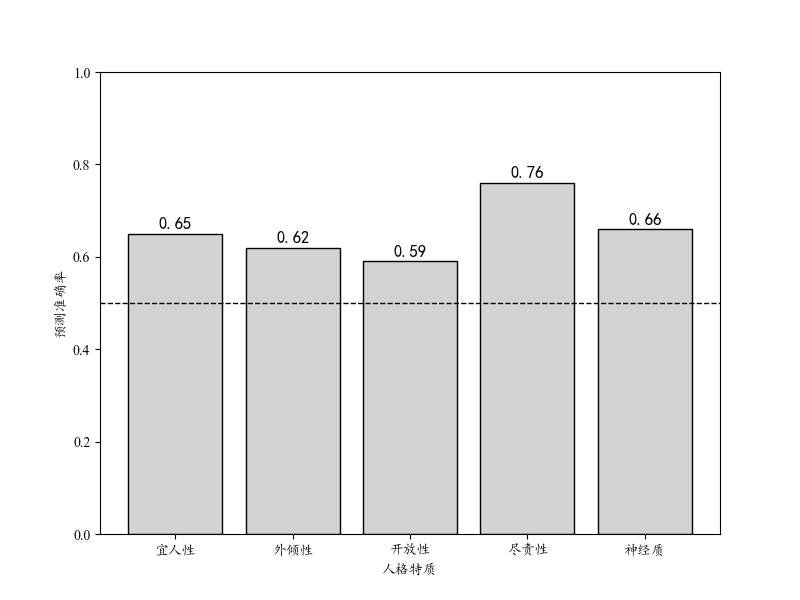
\includegraphics[width=1\linewidth]{Image/Study3-predictionAccuray.png}
    \caption{\label{fig:prediction_accuracy}模型预测准确率}
\end{figure}

为进一步解析个性化广告预测模型中语言特征的作用,本研究引入 SHAP(SHapley Additive exPlanations) 方法对特征贡献进行分析。SHAP 是一种基于 Shapley 值的模型解释方法,被广泛用于评估机器学习模型中各特征对预测结果的贡献。其核心思想是计算每个特征在不同预测情境下的边际贡献,从而提供一致且可解释的特征重要性衡量标准。相比于传统的特征重要性计算方法(如随机森林中的 Gini 重要性或基于置换的重要性分析),SHAP 具有更强的理论可解释性,能够有效捕捉特征间的交互效应,使研究者能够更全面地理解模型的决策过程。

\textbf{(2)特征贡献度}

在本研究中,我们针对五种人格特质(宜人性、外倾性、开放性、尽责性、神经质)分别计算 SHAP 值,以解析不同语言特征在个性化广告预测任务中的贡献。SHAP 值的正负表示该特征对模型预测结果的影响方向:正 SHAP 值表示该特征增加了高水平特质个体偏好的预测概率,而负 SHAP 值则表示该特征更倾向于预测低水平特质个体的偏好模式。此外,SHAP 值的绝对大小反映了该特征的重要性,即数值越大,说明该特征对模型预测的影响越显著。图 \ref{fig:featureHeatmap} 展示了 SHAP 计算得到的特征重要性热力图,横轴表示人格特质类别,纵轴为 LIWC 语言特征,颜色深浅表示该特征在相应人格特质预测任务中的贡献大小。

从 SHAP 计算结果来看,不同人格特质的个性化广告在语言特征上表现出一定的模式。例如,在 \textbf{尽责性} 个性化广告的预测模型中,\textit{drives}(动机相关)、\textit{work}(工作相关)和\textit{quant}(数量表达)等特征的重要性最高,这与尽责性个体强调目标导向、任务执行和条理性的特点一致。同时,\textit{negemo}(负面情绪)特征在尽责性广告预测中也表现出较高 SHAP 贡献,这可能是由于尽责性个体在广告内容中更关注潜在风险或任务挑战,从而影响其对广告的接受度。

在 \textbf{外倾性} 个性化广告的预测模型中,\textit{social}(社交相关)、\textit{posemo}(正面情绪)和\textit{reward}(奖励)等特征的重要性较高,表明外倾性个体更倾向于被强调社交互动、正向体验和激励机制的广告所吸引。此外,\textit{you}(第二人称代词)的贡献也较大,可能表明外倾性个体更偏好直接互动式的广告表达。

\textbf{宜人性} 个性化广告的预测模型则显示,\textit{compare}(比较)、\textit{motion}(运动相关)和\textit{feel}(情感相关)等特征的重要性较高。这表明宜人性个体在广告中更关注人与人之间的关系、情感共鸣以及相对评价,而\textit{pronoun}(代词)的贡献也说明宜人性广告可能更倾向于使用第一人称或第三人称代词,以增强广告的亲和力和人际互动。

\textbf{神经质} 个性化广告的预测模型中,\textit{negemo}(负面情绪)、\textit{tentat}(不确定性)和\textit{risk}(风险)等特征的重要性最高。这表明神经质个体更倾向于受到涉及焦虑、不安和不确定性表达的广告影响,同时也可能偏好那些能够提供安全感和情绪安抚的信息。此外,\textit{social}(社交相关)特征在神经质个体的广告预测中也具有较高贡献,这可能是由于该群体更容易受到社交焦虑或社交互动内容的影响。

相比之下,\textbf{开放性} 个性化广告的预测模型中,各特征的 SHAP 贡献较为分散,缺乏单一主导特征。这可能与开放性人格本身的语言风格高度多样化有关。例如,\textit{informal}(非正式表达)、\textit{cause}(因果逻辑)、\textit{cogproc}(认知过程)和\textit{compare}(比较)等特征在开放性广告预测中均有所贡献,但整体重要性不如其他人格特质广告任务中的显著。这一结果可能表明,开放性广告的个性化表达方式较为宽泛,使得模型难以精准捕捉统一的语言模式。

综合来看,SHAP 分析进一步支持了 LIWC 语言特征在个性化广告预测中的作用,并揭示了不同人格特质在语言表达上的独特性。尽责性、外倾性和宜人性广告的语言特征较为稳定,使得模型能够较准确地预测个性化广告效果,而开放性广告由于语言多样性较高,可能导致预测性能的下降。这一发现不仅为 AI 生成个性化广告的优化提供了数据支持,也为未来在个性化广告设计中更精细地调整语言策略提供了理论依据。

\begin{figure}[H]
    \centering
    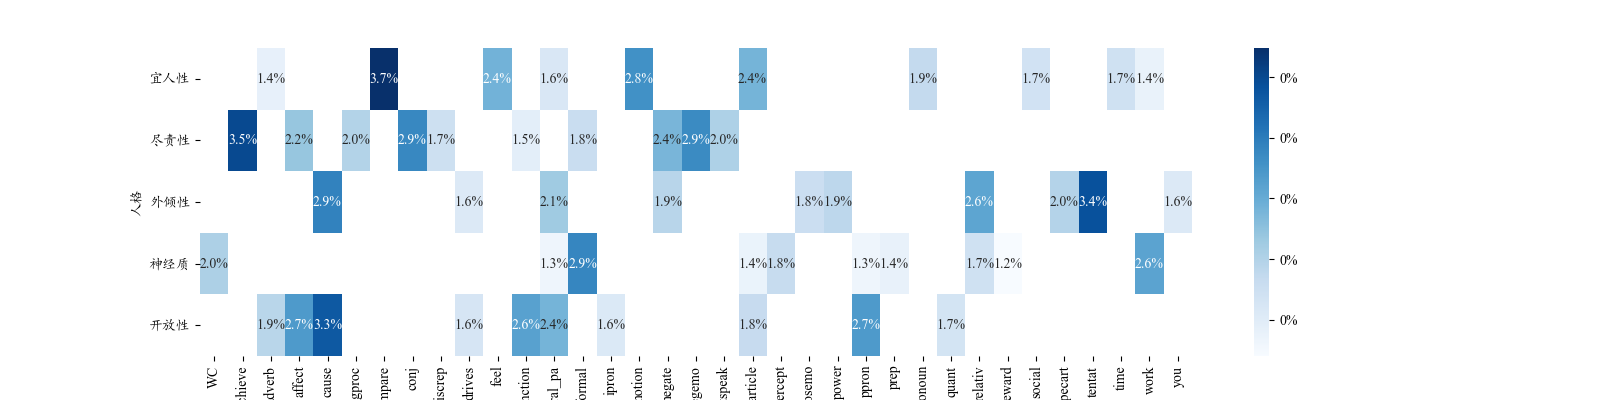
\includegraphics[width=1.2\linewidth]{Image/Study3-heatmap.png}
    \caption{\label{fig:featureHeatmap}特征SHAP值热力图}
\end{figure}

\textbf{(3)高水平vs低水平偏好特征差异}

在本研究中,我们基于参与者的实际广告评分计算了个性化说服效应(计算方法详见 \ref{calculationMethods}),衡量不同人格特质水平的个体对广告内容的偏好模式。相较于子研究一仅关注高水平特质广告文本的语言特征(§ \ref{study3-substudy1}),本研究中进一步分析高低水平人格特质个体在广告语言特征上的偏好差异。通过独立样本t检验比较高水平与低水平个体在LIWC 语言特征偏好上的显著性差异,并计算 Cohen’s d以评估效应量。这一分析不仅揭示了高低水平个体在广告接受度上的语言特征偏好,还为优化个性化广告的匹配策略提供了新的视角。

高宜人性个体更偏好包含 \textbf{比较(compare)} 词汇的广告 \((t = 3.13, p = 0.002, d = 0.59)\),并且在\textbf{代词(pronoun)} 使用上显著更高 \((t = 2.65, p = 0.009, d = 0.50)\)。这表明,高宜人性个体更倾向于接受\textbf{强调个体差异、相对优势} 的广告,例如:“你的时间宝贵,所以我们的手机不容许任何延误。一键快速响应,确保每一秒都计算得刚刚好。” 此外,高宜人性个体对\textbf{未来导向(focusfuture)} 的内容表现出更高的接受度 \((t = 1.97, p = 0.052, d = 0.37)\),说明他们更偏好\textbf{强调长期利益和积极愿景} 的广告表达。低宜人性个体更偏好\textbf{否定(negate)} \((t = -2.04, p = 0.044, d = -0.39)\) 和\textbf{愤怒(anger)} \((t = -2.01, p = 0.049, d = -0.39)\),表明他们对\textbf{直接、批判性更强的广告} 反应更积极,如:“你的朋友已为此狂热,这不仅是手机,更是社交的新纪元。展现个性,享受交流,无限精彩尽在掌中。” 此外,低宜人性个体对\textbf{生物相关词汇(bio,如“健康”“身体”)} 更敏感 \((t = -2.15, p = 0.035, d = -0.42)\),这可能意味着他们更容易被\textbf{与身体机能、健康维护相关的广告} 吸引,如:“智能调节屏幕色温,缓解视疲劳,让工作休闲更加舒适。”

高开放性个体在\textbf{代词(ppron)} \((t = 2.91, p = 0.004, d = 0.55)\) 和\textbf{功能词(function words)} \((t = 2.26, p = 0.026, d = 0.43)\) 的使用上显著更高,表明他们更倾向于接受\textbf{强调个体体验、社交互动,或富有思辨性的广告表达},例如:“使用这款手机,你将体验到最全新的技术、最前卫的设计;在这里,你将以从未想象过的方式探索手机的世界。” 此外,高开放性个体更偏好\textbf{强调集体归属感} 的语言,他们更常被包含 \textbf{“我们”(we)} 的广告所吸引 \((t = 2.06, p = 0.042, d = 0.39)\),如:“共同追求进步,创造美好的明天。手机作为你的工具,与你一同实现梦想。” 低开放性个体更偏好\textbf{数字(number)} \((t = -1.93, p = 0.058, d = -0.36)\),说明他们更倾向于\textbf{基于数据、事实支撑的广告},例如:“99\% 的用户推荐,实验数据显示出色性能。”

高尽责性个体更偏好\textbf{功能词(function)} \((t = 2.70, p = 0.008, d = 0.52)\) 和\textbf{未来导向(focusfuture)} \((t = 1.83, p = 0.070, d = 0.34)\),表明他们更容易接受\textbf{逻辑清晰、目标导向的广告},例如:“精准定位,发现生活中的美好细节。捕捉时刻,记录珍贵瞬间。” 低尽责性个体更偏好\textbf{否定(negate)} \((t = -2.54, p = 0.013, d = -0.50)\) 和\textbf{负面情绪词汇(negemo)} \((t = -2.46, p = 0.016, d = -0.47)\),说明他们更容易被\textbf{强调挑战、失败或压力} 的广告吸引,如:“如果你不立即采取行动,你可能会错失机会。”

高外向性个体更偏好\textbf{相对性词汇(relativ,如“更快”“更高”)} \((t = 2.58, p = 0.011, d = 0.49)\) 和\textbf{不确定性表达(tentat,如“可能”)} \((t = 2.45, p = 0.016, d = 0.46)\),他们更容易接受\textbf{强调探索性、互动感的广告},如:“翻阅朋友的动态,把温馨的友情牢牢捕捉。” 低外向性个体 更偏好\textbf{权力(power)} 相关词汇 \((t = -2.08, p = 0.041, d = -0.40)\),表明他们更倾向于\textbf{强调掌控感、决策权威性的广告},如:“你的时间宝贵,所以我们的手机不容许任何延误。”

高神经质个体偏好\textbf{网络用语(netspeak)} \((t = 2.00, p = 0.050, d = 0.40)\),表明他们更容易接受\textbf{非正式、口语化的广告风格},如:“在欢笑中,她是你探索世界的桥梁;在泪水中,她是你疗愈伤痕的港湾。” 低神经质个体更偏好\textbf{未来导向(focusfuture)} \((t = -3.03, p = 0.003, d = -0.57)\),这表明他们更倾向于\textbf{强调长期规划、稳定性的广告},如:“开启智慧生活,助你成为更好的自己。”

\section{讨论} 

本研究通过文本分析和预测建模,深入探讨了个性化广告文本的语言特征及其对广告说服效果的影响。研究三的结果表明,不同人格特质的个性化广告在语言风格上存在系统性差异 \citep{koutsoumpis2022kernel},且这些差异能够有效预测广告的个性化说服效果。此外,本研究进一步比较了 AI 生成的个性化广告文本特征 与 不同人格特质个体在实际偏好中表现出的语言特征,揭示了 AI 在个性化广告生成中的局限性。尽管 AI 在广告设计时基于各特质的语言风格进行针对性优化,但由于语言使用在不同情境下可能呈现不同特征,即使是同一人格特质,针对不同广告类型,其语言风格也可能存在显著差异 \citep{flores2014effect},AI 在个性特质与广告场景的结合方面仍然存在短板。此外,以往研究主要关注高水平特质的语言偏好,而对低水平特质的个性化偏好探讨较少,本研究的结果表明,低水平特质个体的广告偏好并不完全符合传统人格特质的解读,而在广告情境下表现出新的特征倾向。例如,某些低水平特质个体偏好的特征与其在一般语言研究中的表现不完全一致,这表明个性化广告的说服机制可能受到额外的语境因素影响。这些发现不仅反映了 AI 生成广告在低水平特质个性化匹配上的挑战,也为未来个性化广告优化提供了新的方向。因此,未来的个性化广告生成需要更加关注语言风格在不同语境中的适应性,并结合高低水平特质的实际偏好,以提高个性化匹配的精准度和广告的说服力。接下来将从各人格特质展开,进一步讨论 AI 生成文本与实际个性化偏好的具体差异,并探讨其可能的成因及优化方向。

在\textbf{外倾性}个性化广告的设计中(如表 \ref{tab:study3_extraversion_comparison}),AI 主要关注的是社交互动、情感表达和积极体验,因此生成的广告文本往往包含大量社交相关(social)和正面情感(posemo)词汇,例如“与世界分享你的热情,记录美好时刻,激发他人的快乐与欢笑”。此外,外倾性广告通常也会使用感知类(percept)词汇,以增强体验感。然而,从外倾性参与者的实际反馈来看,尽管这些元素符合外倾性个体的语言风格,但更能提升个性化广告效果的特征还包括激励性表达(reward)和互动性用语(you),如“你的朋友已为此狂热,这不仅是手机,更是社交的新纪元”。相比之下,AI 在生成广告时虽然强调了社交主题,但可能低估了“互动”在广告场景中的重要性。造成这一偏差的一个可能原因是,大多数关于人格与语言的研究侧重于个体的自然语言表达习惯,而不是他们在广告情境下的偏好。外倾性个体的日常语言确实包含更多社交词汇,但这些表达通常是针对社交情境,而非广告语境。在广告场景中,外倾性个体可能更倾向于被直接卷入对话,需要更多“你”(you)的参与感,而不仅仅是对“社交”概念的描述。因此,AI 在广告生成时,应考虑如何从社交语言风格转向“交互式”语言设计,例如采用问题导向、邀请式的表达(如“你将如何使用这款手机?”),以进一步增强广告的吸引力。此外,低外倾性个体的广告偏好与传统外倾性/内倾性语言风格的理解并不完全一致。通常,低外倾性个体在自然语言表达中更偏向于内省、个体化、秩序感,但在广告场景下,他们更倾向于强调权力和掌控感的广告,如“精准管理你的时间,高效完成每一个任务”。这可能表明他们对社交互动的关注度较低,而更希望广告提供增强个人自主性的承诺。这与研究发现的低外倾性个体更喜欢反思、更注重个体控制,并倾向于结构化和秩序化的生活一致 \citep{beukeboom2013language}。这一发现说明,在个性化广告的设计上,AI 不应仅停留在基于人格特质的表层语言特征,而应深入挖掘不同人格特质的更深层次需求,特别是在特定广告情境下如何有效激发不同群体的兴趣和认同感。


\begin{table}[H]
    \centering
    \caption{\label{tab:study3_extraversion_comparison} 高外倾与低外倾的个性化广告语言特征偏好}
    {\tablesongti % 整个表格环境应用宋体六号字体
    \renewcommand{\arraystretch}{1.5} % 调整行距
    \begin{tabularx}{\linewidth}{l X X} % 设定每列宽度
        \toprule
        \textbf{外倾性} & \textbf{AI 生成} & \textbf{实际偏好} \\
        \midrule
        \multirow{5}{*}{\textbf{高外倾}} 
        & 社交相关(social),如“与世界分享你的激情” & 社交相关(social),如“你的朋友已为此狂热” \\
        & 正面情感(posemo),如“让你的社交世界明亮而充满希望” & 正面情感(posemo),如“激发他人的快乐与欢笑” \\
        & 感知体验(percept),如“感受科技带来的精彩” & 感知体验(percept),如“探索全新体验” \\
        &  & \textcolor{red}{互动性(you),如“你将如何使用?”} \\
        &  & \textcolor{red}{激励性表达(reward),如“开启你的无限可能”} \\
        \midrule
        \multirow{5}{*}{\textbf{低外倾}} 
        & \multirow{5}{*}{样本不足未分析}  & 强调个人自主(individuality),如“精准管理你的时间” \\
        &  & 掌控感(control),如“助你高效决策” \\
        &  & 秩序、结构化表达(order),如“让你的生活井然有序” \\
        &  & 权力(power),如“主宰你的生活节奏” \\
        \bottomrule
    \end{tabularx}
    }
\end{table}


在\textbf{宜人性}个性化广告的设计上(如表 \ref{tab:study3_agreeableness_comparison}),AI 主要强调温暖、关怀和归属感,因此生成的广告往往包含较多积极情感(posemo)、社交相关(social)和归属动机(affiliation)词汇,如“用这款手机,把温情传递给每一个需要的角落”。然而,实际广告偏好表明,他们还更加看重比较性表达(compare)和未来导向(focusfuture),例如“精准生活,从不间断”。这一点可能源于高宜人性个体在社交互动中不仅关注情感连接,还关注相对优势和长远利益,他们希望看到广告内容如何凸显产品在人际关系或个人体验中的独特性。这一偏好与以往研究对宜人性个体的理解有所不同,因为过往研究多强调宜人性与和谐沟通的关系,而本研究的结果表明,在广告场景中,高宜人性个体更关注产品的竞争力,以及产品如何带来持续性的价值。而对于低宜人性个体,在实际偏好中更倾向于直接、批判性更强的语言风格,如否定性表达(negate)和愤怒(anger)。此外,他们还对生物相关内容(bio) 产生了更高的偏好,这表明低宜人性个体可能更关注产品对个人生理需求的直接影响,而不是对社交关系的促进。这与传统研究强调低宜人性个体更直接较少关注情感交流和他人感受的特征一致 \citep{crowe2018uncovering}。未来的个性化广告设计应考虑,针对低宜人性个体,广告可以减少冗余的情感表达,而更加强调产品的物理性能、个人体验和问题解决能力,例如“强劲性能,不再忍受卡顿”或“守护你的健康,关心你的身体”。

\begin{table}[H]
    \centering
    \caption{\label{tab:study3_agreeableness_comparison} 高宜人性与低宜人性的个性化广告语言特征偏好}
    {\tablesongti % 整个表格环境应用宋体六号字体
    \renewcommand{\arraystretch}{1.5} % 调整行距
    \begin{tabularx}{\linewidth}{l X X} % 设定每列宽度
        \toprule
        \textbf{宜人性} & \textbf{AI 生成} & \textbf{实际偏好} \\
        \midrule
        \multirow{4}{*}{\textbf{高宜人性}} 
        & 积极情感(posemo),如“用这款手机,把温情传递给每一个需要的角落” & 积极情感(posemo),如“用这款手机,把温情传递给每一个需要的角落” \\
        & 社交相关(social),如“记录美好瞬间,让善意的温暖传递到每个角落” & 社交相关(social),如“记录美好瞬间,让善意的温暖传递到每个角落” \\
        & 归属动机(affiliation),如“与世界分享你的温暖,让每一次沟通都更有意义” &  \textcolor{red}{比较(compare),如“精准生活,从不间断”} \\
        & &  \textcolor{red}{未来导向(focusfuture),如“开启你的无限可能”}  \\
        \midrule
        \multirow{4}{*}{\textbf{低宜人性}} 
        & \multirow{4}{*}{样本不足未分析} \\
        & & 直接性表达(directness),如“告别卡顿死机” \\
        & & 否定(negate),如“再也不用担心电池续航” \\
        & & 愤怒(anger),如“强劲性能,不再忍受卡顿” \\
        & & 生物相关(bio),如“守护你的健康,关心你的身体” \\
        \bottomrule
    \end{tabularx}
    }
\end{table}


在\textbf{尽责性}的个性化广告设计中 (\ref{study3_conscientiousness_comparison}),AI 主要强调目标导向、条理性和成就感,因此生成的广告文本通常包含较多成就动机(achieve)、数量表达(quant) 以及长词(sixltr),如“精准管理你的日常,高效提升你的生产力。” 这些特征确实符合高尽责性个体的语言风格,但从实际偏好来看,他们更倾向于逻辑清晰的功能描述(function) 和 未来导向表达(focusfuture),如“掌控你的时间,高效完成每一个任务。” 这一发现表明,高尽责性个体不仅关注广告是否强调成就和效率,还更希望广告能提供清晰的目标实现路径。然而,AI 在广告生成时通常更偏向于静态描述,强调“提升效率”或“提高生产力”,而忽略了如何实现这一目标的具体行动步骤。造成这一偏差的一个可能原因是,AI 主要基于语言风格匹配,而非深度建模尽责性个体的思维模式。尽责性个体通常偏好结构化的因果逻辑,即如何从当前状态迈向未来目标,但 AI 生成的广告语料主要受商业营销策略影响,过度依赖数据支持(quant)和成就动机(achieve),而缺乏因果推理(cause)。例如:AI 当前生成:“每天提升 20\% 的工作效率。” 高尽责性个体可能更偏好:“通过智能计划和任务提醒,帮助你每天提升 20\% 的工作效率。” 此外,分析得到低尽责性个体偏好的广告特征是带有紧迫感或挑战性的广告,如“如果你不立即采取行动,你可能会错失机会”。这与低尽责性个体的心理特质相一致,他们往往缺乏长期规划能力,更容易受到即时刺激和情境驱动的影响 \citep{deyoung2010impulsivity}。

\begin{table}[H]
    \centering
    \caption{\label{tab:study3_conscientiousness_comparison} 高尽责与低尽责的个性化广告语言特征偏好}
    {\tablesongti % 整个表格环境应用宋体六号字体
    \renewcommand{\arraystretch}{1.5} % 调整行距
    \begin{tabularx}{\linewidth}{l X X} % 设定每列宽度
        \toprule
        \textbf{尽责性} & \textbf{AI 生成} & \textbf{实际偏好} \\
        \midrule
        \multirow{5}{*}{\textbf{高尽责性}} 
        & 目标导向(achieve),如“精确管理你的日常,高效提升你的生产力” & \textcolor{red}{逻辑清晰的功能描述(function),如“通过智能计划和任务提效,帮助你每天提高 20\% 的工作效率”} \\
        & 数量表达(quant),如“提升 20\%的效率” & \textcolor{red}{未来导向表达(focusfuture),如“掌控你的时间,高效完成每一个任务”} \\
        & 长词使用(sixltr),语言更正式、结构化 & \textcolor{red}{因果推理(cause),如“高效计划每一天,从目标设定到成果实现”}\\
        \midrule
        \multirow{5}{*}{\textbf{低尽责性}} 
        & \multirow{5}{*}{样本不足未分析} \\
        &  & 紧迫感(urgency),如“如果你不立即采取行动,你可能会错失机会”\\
        &  & 挑战性(challenge),如“现在就抓住住机会!”\\
        &  & 非正式表达(informal),如“快来试试,让生活更轻松!”\\
        \bottomrule
    \end{tabularx}
    }
\end{table}


在\textbf{开放性}广告的设计中(表\ref{tab:study3_openness_comparison}),AI 主要关注探索性、创造性和认知加工,因此生成的广告往往包含较多认知加工(cogproc)、洞察(insight)和空间感知(space)词汇,如“探索这款手机,感受尖端科技与前卫设计的融合”。这些特征符合开放性个体在语言使用上更倾向于抽象概念和认知探索的特点 \citep{deyoung2014openness},然而,实际个性化广告的测试结果显示,因果逻辑(cause)和非正式表达(informal)可能在广告说服过程中更具影响力,例如“你的世界,由你定义”这样的表达比单纯的探索性描述更有效。值得注意的是,因果逻辑的偏好与前人文献的结论相反\citep{pennebaker1999linguistic}。以往研究认为,高开放性个体的语言风格更倾向于发散性思维,具有更高的抽象性和创造性,因而可能更偏好非线性、开放式的表达。然而,本研究的发现表明,在广告语境中,当广告内容涉及个性化说服时,高开放性个体更容易关注信息的逻辑性,而非单纯的抽象表达。这可能是因为广告本质上是一种说服性沟通,个性化广告的匹配过程可能会促使受众进行更深层次的认知加工(deliberate processing),而在这一过程中,因果关系明确的句子能够提供清晰的推理路径,使高开放性个体更容易理解广告的核心价值。例如,相较于“解锁你的创造力,探索无限可能”这种较为模糊的表达,高开放性个体在广告评价中更青睐“通过 AI 影像增强技术,让你的创意变得更清晰”,因为后者提供了明确的因果关系,增强了信息的可理解性和可信度。此外,本研究还发现,高开放性个体在广告中更偏好非正式表达(informal),这一点与高开放性个体更倾向于接受个性化、随性的表达方式的特点一致。研究表明,在创意广告中,带有幽默或非正式元素的广告更能够激发灵活思维和创造力 \citep{kover1995creativity},更符合高开放性个体对新颖性和独特性的偏好。例如,“嘿,你准备好迎接一款真正与众不同的手机了吗?” 这样的非正式语句可能比“本产品将带来创新性的使用体验”更能引起高开放性个体的兴趣。相比之下,AI 生成的广告文本更多采用正式、标准化的表达,而在未来的优化方向中,可以进一步融入更加个性化、随性且富有创造力的非正式表达,以提升对高开放性个体的吸引力。在低开放性个体的个性化偏好中,本研究发现他们更倾向于数据驱动和事实支撑的信息,例如“99\% 的用户推荐”或“实验数据显示,这款产品性能提升 20\%”;以及低对确定性(certainty)和稳固性(stability)的需求,例如“经过验证,这款手机更加稳定可靠”,这与低开放性更倾向于可预测、可靠产品的特点相符。

\begin{table}[H]
\centering
\caption{\label{tab:study3_openness_comparison} 高低开放性个体的AI 生成特征与实际偏好特征对比}
{\tablesongti
\renewcommand{\arraystretch}{1.5} % 调整行距
\begin{tabularx}{\linewidth}{l X X} % 设定每列宽度
    \toprule
    \textbf{开放性} & \textbf{AI 生成} & \textbf{实际偏好} \\
    \midrule
    \multirow{4}{*}{\textbf{高开放性}} 
    & 认知加工(cogproc),如“探索这款手机,感受尖端科技与前卫设计的融合” & 认知加工(cogproc),如“你的世界,由你定义” \\
    & 洞察(insight),如“打开新的可能,创造属于你的未来” & \textcolor{red}{因果逻辑(cause),如“先进技术让使用体验更加流畅”} \\
    & 空间感知(space),如“广阔视野,让探索无界” & \textcolor{red}{非正式表达(informal),如“随时随地,想拍就拍”} \\
    &  & \textcolor{red}{集体归属(we),如“共同追求进步,创造美好的明天”} \\
    \midrule
    \multirow{4}{*}{\textbf{低开放性}} 
    & \multirow{4}{*}{样本不足未分析}\\
    &  & 数据驱动(number),如“99\% 的用户推荐” \\
    &  & 确定性(certainty),如“经过验证,这款手机更加稳定可靠” \\
    &  & 稳固性(stability),如“专业测试认证,确保长期使用稳定” \\
    \bottomrule
\end{tabularx}
}
\end{table}


在\textbf{神经质}个性化广告的设计中(如表\ref{tab:study3-neuroticism_comparison}),AI 主要关注情绪波动和安全感,因此生成的广告往往包含较多负面情感(negemo)、焦虑(anx)、愤怒(anger)和悲伤(sad)词汇,如“在泪水中,她是你疗愈伤痕的港湾”。这些表达与高神经质个体的典型语言风格一致,符合他们对情绪相关信息更敏感的特点。然而,实际偏好分析显示,高神经质个体更倾向于非正式表达(netspeak)和即时满足(reward),如“在快节奏的生活中,找到一个真正与你同步的伴侣”。相比之下,AI 低估了这些因素在个性化广告中的作用。这可能源于神经质个体在自然语言表达和广告接受偏好上的差异——虽然他们的语言风格通常表现出高情绪性,但他们在广告中更偏好具有亲和力、轻松随性的表达方式,而不是强化负面情绪。例如,非正式表达可以减少广告对焦虑个体的威胁性,使广告更具可接受性,而即时满足的承诺则能够降低不确定性,为他们提供即时的情绪安抚 \citep{miller2006neuroticism}。因此,AI 在优化神经质广告时,不应仅关注情绪化表达,而应结合更轻松、互动式的语言,提供更直接的情绪补偿和安全感承诺。在低神经质个体的个性化偏好中,本研究发现他们更倾向于长期规划(focusfuture)和稳定性(stability)的表达,例如“开启智慧生活,助你成为更好的自己”或“经过时间验证,依然强大稳定”。这与他们更低的情绪不稳定性和更高的心理韧性一致。相比高神经质个体的即时满足倾向,低神经质个体更能接受延迟满足,因此强调未来利益的广告对他们更具吸引力。此外,他们也较少受到情绪化信息的影响,更倾向于理性、务实的语言风格。因此,在个性化广告设计中,针对低神经质个体的广告应避免情绪性夸张,而是强调稳定、可靠的产品优势,并通过明确的未来规划信息增强广告的说服力。高低神经质的个性化偏好在过往文献中常无法得到有效的结果,个体的实际偏好差异,表明在广告个性化策略上,不能仅依据神经质个体在自然语言中的情绪表达风格,而应结合广告的实际作用机制进行调整。高神经质个体的广告需要减少焦虑诱发因素,并提供即时情绪安抚,而低神经质个体则更偏好稳定、长期规划的信息结构。未来的个性化广告优化可以进一步结合情绪调节策略,使广告内容不仅与个体语言风格匹配,也能够针对个体心理需求进行精准调整。以往文献发现,高低神经质个体的广告接受偏好并不像其他人格特质那样容易区分 \citep{matz2024potential},部分原因在于高神经质个体不仅关注情绪共鸣,也渴望获得缓解焦虑的方式,而低神经质个体对情绪内容的接受度较高,但更偏好清晰的事实信息。因此,未来的个性化广告优化应进一步结合个体的情绪调节需求,针对高神经质个体减少焦虑诱发因素,提供即时满足的信息,而针对低神经质个体则强调长期规划和稳定性,使广告内容能够更精准地适应不同个体的心理需求。

\begin{table}[H]
\centering
\caption{\label{tab:study3-neuroticism_comparison} 高低神经质个体的AI 生成特征与实际偏好特征对比}
{\tablesongti
\renewcommand{\arraystretch}{1.5} % 调整行距
\begin{tabularx}{\linewidth}{l X X} % 设定每列宽度
    \toprule
    \textbf{神经质} & \textbf{AI 生成} & \textbf{实际偏好} \\
    \midrule
    \multirow{2}{*}{\textbf{高神经质}} 
    & 负面情感(negemo),如“在泪水中,她是你疗愈伤痕的港湾” & \textcolor{red}{非正式表达(netspeak),如“在快节奏的生活中,找到一个真正与你同步的伴侣”} \\
    & 焦虑(anx)、愤怒(anger)、悲伤(sad)词汇,突出情绪波动 & \textcolor{red}{即时满足(reward),如“开启无限可能,即刻体验”} \\
    \midrule
    \multirow{2}{*}{\textbf{低神经质}} 
    &  \multirow{2}{*}{样本不足未分析} \\
    &  & 长期规划(focusfuture),如“开启智慧生活,助你成为更好的自己” \\
    &  & 稳定性(stability),如“经过时间验证,依然强大稳定” \\
    \bottomrule
\end{tabularx}
}
\end{table}


本研究通过对 AI 生成的个性化广告文本与不同人格特质个体的实际偏好进行比较,揭示了 AI 在广告生成中的局限性:语言使用的场景适应性不足、个性化策略的刻板化。尽管 AI 生成的广告在一定程度上能够匹配目标特质的语言风格,但语言风格的匹配并不必然等同于广告的高效说服力。广告作为一种具有特定传播目的的信息载体,其个性化策略不仅需要精准表达目标特质,还需兼顾广告语境的适应性,以及受众在信息加工过程中的认知与情感需求。针对这一问题,未来 AI 生成个性化广告的优化方向需要从单纯的语言风格匹配拓展至更深层次的语境适配性。具体而言,AI 在个性化广告生成时,不应仅关注受众在自然语言中的表达习惯,还需识别特定广告场景下语言使用的实际功能。例如,即便某些语言特征在日常交流中较为常见,它们在广告语境下的有效性仍可能受到受众信息处理模式的影响。不同广告目标(如品牌塑造、产品推广、情感共鸣等)对语言风格的要求不同,AI 需要在个性化表达与广告实际传播效果之间找到平衡,使个性化不仅体现在语言特征的匹配上,更体现在广告说服力的提升上。这不仅为个性化广告优化提供了新的实证支持,也为 AI 在广告创作中的应用提出了新的优化方向。

